\documentclass{bioinfo}
\copyrightyear{2015} \pubyear{2015}

\access{Advance Access Publication Date: Day Month Year}
\appnotes{Manuscript Category}
\usepackage{url}

% extra counters to reference items in supplemental
% note that thes are not directly linked, so the order of the environments 
% should match where they occur in the supplement
\newcounter{supfig}
\newenvironment{supfig}[1][]{\refstepcounter{supfig}}

\newcounter{suptab}
\newenvironment{suptab}[1][]{\refstepcounter{suptab}}

\newcounter{supsec}
\newenvironment{supsec}[1][]{\refstepcounter{supsec}}

\newcounter{supdata}
\newenvironment{supdata}[1][]{\refstepcounter{supdata}}


\begin{document}
\firstpage{1}

\subtitle{Genome analysis}

\title[short Title]{Helixer: Cross-species Gene Annotation Of Large Eukaryotic Genomes Using Deep Learning}
\author[Sample \textit{et~al}.]{Felix Stiehler\,$^{\text{\sfb 1}}$, Marvin Steinborn\,$^{\text{\sfb 1}}$, Stephan Scholz, Daniela Dey\,$^{\text{\sfb 2}}$, Andreas P.M. Weber\,$^{\text{\sfb 1}}$, Alisandra K. Denton\,$^{\text{\sfb 1,}*}$}
\address{$^{\text{\sf 1}}$Institue of Plant Biochemistry, Heinrich-Heine-University, Dusseldorf, 40225, Germany\\
$^{\text{\sf 2}}$Institute of Human Genetics, Medical Faculty, RWTH Aachen University, Aachen, 52062, Germany}

\corresp{$^\ast$To whom correspondence should be addressed.}

\history{Received on XXXXX; revised on XXXXX; accepted on XXXXX}

\editor{Associate Editor: XXXXXXX}

\abstract{
\textbf{Motivation:} Current state-of-the-art tools for the \textit{de novo} annotation of 
genes in eukaryotic genomes have to be specifically fitted for each species and still often 
produce annotations that can be improved much further. The fundamental algorithmic 
architecture for these tools has remained largely unchanged for about two decades, limiting
learning capabilities. Here, we set out to improve the cross-species annotation of
genes from DNA sequence alone with the help of deep learning. The goal is to eliminate 
the dependency on a closely related gene model while also improving the predictive
quality in general with a fundamentally new architecture.\\
\textbf{Results:} We present Helixer, a framework for the development and usage of 
a cross-species deep learning model that improves significantly on performance and
generalizability when compared to more traditional methods. We evaluate our 
approach by building a single model for the annotation of 186 animal genomes as 
well as one for 51 plants. Our predictions are shown to be much less sensitive to
the length of the genome than those of a current state-of-the-art tool. We also 
present two novel post-processing techniques that each worked to further strengthen 
our annotations and show in-depth results of an RNA-Seq based comparison of our 
predictions.\\
\textbf{Availability:} The source code of this work is available at 
\url{https://github.com/weberlab-hhu/Helixer} under the GNU General 
Public License v3.0.\\
\textbf{Contact:} \href{alisandra.denton@hhu.de}{alisandra.denton@hhu.de}\\  
\textbf{Supplementary information:} Supplementary data are available at 
\textit{Bioinformatics} online.
}

\maketitle

\section{Introduction}
Annotating genes is an integral part of
genomic DNA sequence analysis, with many downstream taks
dependent on annotation quality.
Gene annotation can be performed at different levels 
of precision, from simple coding -- non-coding classification to detailed structural 
labeling. Because of the sheer size of genomes alone, manual gene annotation is 
generally intractable. Instead, researchers can use pipelines such as 
Maker \citep{cantarel2008maker}, PASA \citep{haas2003improving} or those 
offered by genomic database providers like NCBI 
\citep{thibaud2013eukaryotic} and Ensembl \citep{aken2016ensembl}. 
These pipelines integrate experimental data (from e.g. RNA-seq 
or proteogenomics) with homologous sequences in the database and ab-initio gene 
predictions. The latter is an attractive approach, because it is cheap and fast. 
State-of-the-art performance is achieved by higher order hidden markov models 
(HMMs), such as Genscan \citep{burge1997prediction}, AUGUSTUS \citep{stanke2003gene} 
or SNAP \citep{johnson2008snap}. Their accuracy, however, leaves room for 
improvement. By encoding possible states and transitions in a probalistic model, 
designers of HMMs assume structure in the sequence that may limit its predictive 
power. In practice HMMs have trouble generalizing across species and the actual learning 
of sequence motifs is limited to very short sequences that indicate state transitions.

In the last decade, deep neural networks (DNN) have been applied with great success 
in many areas of statistical modelling, including biology 
\citep{ching2018opportunities}. For sequence data, such as DNA, speech or text, a 
special kind of recurrent neural network (RNN) called long-short term memory (LSTM) 
\citep{hochreiter1997long} is an established building block for many different 
architectures. LSTM units can also be used to process sequential input starting 
from both ends, forming a bidirectional LSTM (BLSTM). It has also been shown that 
HMMs can be successfully combined with DNNs \citep{liu2016novo, liu2016pedla}.

For the purpose of gene annotation, RNNs have already shown promising results. 
\citep{choudharypredicting} carries out preliminary explorations on the potential 
of BLSTMs for cross species gene prediction and trains his model on human genes to 
test it later on two more species. DeepAnnotator \citep{amin2018deepannotator} uses 
BLSTMs for gene finding in prokaryotes. Gene prediction in 
prokaryotes is considered more amenable than in eukaryotes, as genes in prokaryotes 
are proportionately more frequent in the genome, feature simpler control structures 
and do not use splicing \citep{wang2004brief}. DanQ \citep{quang2016danq} proposes 
the use of a BLSTM after a convolutional neural net (CNN) to find detailed motifs in 
the human genome. DeePromoter \citep{oubounyt2019deepromoter} trains a similar 
architecture for the recognition of promoter regions. Recently, several groups 
\citep{jaganathan2019predicting, wang2019splicefinder} successfully used CNNs to 
find splicing sites.

In this work we present Helixer, a novel prototype software for training and 
utilizing a general purpose DNN for the ab-initio cross-species gene annotation of 
large eukaryotic genomes using only DNA sequence as input. Our model is trained to 
differentiate between 4 regions: Intergenic, Untranslated (UTR), Coding (CDS) and 
Intron. We demonstrate the effectiveness of this approach by training a single model 
for the annotation of a large set of genomes from the kingdoms metazoa and 
viridiplantae, respectively, which we will call {\it animals} and {\it plants} from 
now on. We worked with the full data of 192 animal genomes and 60 plant genomes. 
Both the ability to generalize across genomes as well as the scope of the evaluation 
represent cutting edge progress in this field. The source code and all input data 
is publicly available.

\begin{methods}
\section{Methods}
\subsection{Datasets}
The foundation of our work are 192 animal and 60 plant genomes. The data of each 
genome consists of the latest publicly available genomic assembly in form of a 
FASTA file and the latest annotation in the GFF format. One genome for each species of animal 
in EnsemblMetazoa 45 (\cite{howe2020ensembl}; Table S\ref{suptab:downloads_animals}) 
as well as all non-embargoed plant species from the JGI Phytosome 13 database 
(\cite{goodstein2012phytozome}; Table S\ref{suptab:downloads_plants}); The exact 
genomes are listed in the aforementioned tables.
Data was downloaded on the 15/10/2019 and 29/03/2019 for animals and plants respectively. 
Both data groups were used separately during training and evaluation. 

At the start of our work we split both genome groups into {\it training genomes} and 
{\it test genomes}. The test genome groups are made up of 19 and 6 genomes, 
respectively, and were chosen to be of decent quality and diversity based on collected 
metadata (see section S\ref{ssec:data_prep} and Dataset S\ref{supdata:metadata}) 
while also representing a broad phylogenetic spread. 

For the selection of training genomes we had to balance multiple conflicting 
trade-offs. On the one hand, we want to train with as much data as possible, but 
on the other
not all data has sufficient quality to enable a powerful generalization. It is 
also very desirable to have diverse training genomes with a broad phylogenetic spread, 
a variety of genome sizes and average gene lengths as the model is increasingly unlikely to generalize 
well beyond the borders given by the training data. However, it also may be difficult 
for the model to learn and generalize if the genomic patterns inside the data are 
too different from each other. Practically, it was important for us to limit the size of
our training genomes set to be small enough that we could get experimental 
results within a couple of days and thereby be able to test many different data and 
model configurations.

We employed an iterative approach to effectively select a proper set of training 
genomes, starting from 3-4 genomes that were expected to be of the 
highest quality. We then evaluated the performance of the resulting model on all 
genomes individually (including the training genomes) and looked for candidates to 
add to the training set or to remove from it. This process was repeated multiple 
times concurrently with the model search until we saw no more room for substantial 
improvement given our computational constraints.

The genomes that were ultimately not used during training from the original 
split are hereafter refered to as the {\it validation genomes}. 
We report only the generalization 
performance on the combined set of validation and test genomes as the validation 
genomes are by far the largest set, and there was not a noticeable difference in 
performance between those two groups. 

Once a set of training genomes was selected, we further split the sequences therein into a {\it 
training and validation set}. This split of the training genomes was done to get a 
quicker sense of the generalization capabilities and was used primarily during 
training. We split off the validation set by selecting 20\% of the FASTA sequences 
above and below the N90 of each training genome at random, ensuring a proper distribution of 
large and short sequences in both sets and a split on the chromosome level. 
Evaluation of the annotations on all training and validation genomes was done 
regularly after a promising model candidate was found based on its validation set 
performance. Ultimately we used the cross-species performance on all 
validation genomes as the decisive measure of model quality.

\subsection{Data Pre-processing}
We first pre-processed and stored the raw genomic information by using GeenuFF 
(https://github.com/weberlab-hhu/GeenuFF). 
GeenuFF is a tool for checking and exploring genomic data and annotations, that 
stores all information inside a SQL database. Training and evaluation-ready data was
generated by querying this database and then transforming the returned data into a 
numerical format suitable for machine learning. The encoding of the genomic sequence 
was done in line with the IUPAC nucleic acid notation and the functional annotation 
used as labels during training is transformed to a one hot encoding with the four 
classes {\it Intergenic}, {\it UTR}, {\it CDS} and {\it Intron}. See Table 
\ref{tab:arrays} for a more detailed description of the generated data types.

\begin{table}[!htb]
\label{tab:arrays}
\processtable{Data arrays generated and used by Helixer}{
\begin{tabular}{@{}ll@{}}
\toprule Name & Information \\
\midrule
Input & Genomic sequence in the 4-dimensional IUPAC encoding\\
	  & (one hot encoding for non-ambiguous bases) \\
Output & Labels in a 4-dimensional one hot encoding representing \\
      & the classes {\it Intergenic}, {\it UTR}, {\it CDS} and {\it Intron}\\
Sample weights & One of $\{0,1\}$; whether there is an error at a base\\
\botrule
\end{tabular}}{{\it Note:} The encoding does not differentiate between introns
in coding and non-coding regions.}
\end{table}

During data generation, we queried for the transcript with the longest protein of each gene and 
disregard FASTA sequences that have no functional annotation as it is ambiguous
whether such sequences contain no genes or 
were simply not annotated in the reference. GeenuFF checks the 
genomic annotations for potential errors during import and is able to mark those 
areas. We used this information to effectively mask those bases during training 
by using the sample weights described in Table \ref{tab:arrays}. The vast majority 
of masked bases lie in the intergenic region as the most prevalent error is a 
missing UTR and GeenuFF marks a potentially large intergenic region for it. Table 
\ref{tab:statistics_all} shows statistics about the masking. 

For the training itself, we divided each continuous genomic sequence into 20,000 bp 
long subsequences, for which one-hot vectors of the base pairs and annotations 
are generated and respectively used as input and label for the neural network 
together with the sample weights. We appended zero padding if the subsequences  
are shorter than 20,000 bp. 
If a subsequence is fully marked as erroneous, we excluded it from all analyses. 

\begin{table}[!htb]
\processtable{Data group statistics for all data\label{tab:statistics_all}} {
\begin{tabular}{@{}lll@{}}
\toprule & Animals & Plants\\
\midrule
Average genome size in Gbp& 2.936 (+- 1.562) & 0.787 (+- 0.995) \\
Average gene length & 31,223 (+- 13,974)& 3,368 (+- 1,510)\\
Geenuff error rate & 0.311 (+- 0.129) & 0.351 (+- 0.249) \\
Fraction of class Intergenic  & 0.777 (+- 0.042) & 0.799 (+- 0.089) \\
Fraction of class UTR & 0.006 (+- 0.006) & 0.017 (+- 0.016) \\
Fraction of class CDS & 0.016 (+- 0.014) & 0.085 (+- 0.071) \\
Fraction of class Intron & 0.201 (+- 0.035) & 0.099 (+- 0.057) \\
\botrule
\end{tabular}}{{\it Note:} Values are averages of the individual values of each 
genome in a data group. All statistics except the average gene lengths exclude
FASTA sequences without a gene and any 20,000 bp subsequences that were masked as completely 
erroneous. Each strand of DNA was counted separately. The gene length was 
determined by the length of the pre-mRNA of the longest protein at each
loci. Brackets show the standard deviation.}
\end{table}


\subsection{Metrics}
\label{sec:metrics}
We mainly used two metrics to judge model performance. The {\it Genic F1} was selected as our 
primary metric and provides the most comprehensive picture of annotation quality 
in one number. The {\it Subgenic F1} is similar to the Genic F1, except that it does 
not take UTR predictions into account. This was calculated for comparability with AUGUSTUS 
as further explained in Section \ref{sec:augustus}. Both metrics work by summing up 
True Positives (TP), False Positives (FP) and False Negatives (FN) of each 
considered class before calculating precision and recall from these values and 
combining the two into a F1 score. Neither metric includes the
intergenic class, as this class is very abundant and appears to be by 
far the easiest to predict. (See Table \ref{tab:statistics_all} for the class 
distribution and Tables S\ref{suptab:generalization_animals} 
and S\ref{suptab:generalization_plants} for a more in-depth report our model performance 
including the intergenic class). In the case of the Genic F1, this means that 
effectively only the TP of the intergenic class were disregarded. The metrics 
essentially provide a weighted mean of the performances in the considered classes,
with weights proportional to class frequency.

In Figure \ref{fig:main_results}c we also report on the overall base pair level 
accuracy besides the Genic F1.

\subsection{Model Architecture and Training}
\label{sec:model}
We used a 4-layer deep stacked BLSTM network with 256 units per layer and layer 
normalization \citep{ba2016layer} between each BLSTM layer to produce the 
predictions in the form of a base pair wise classification. The model consists of 
circa 5.4 million parameters and was implemented with the deep learning library 
Keras (https://keras.io) on top of TensorFlow \citep{abadi2016tensorflow}. We 
tested multiple different architectures before arriving at this model configuration, 
including convolutional neural networks (CNN) and hybrid architectures. We also used 
class weights as the class frequencies are both unbalanced and 
vary greatly between animals and plants. 
For example, the trade-off between the number of intergenic and intronic bases is 
quite different in both groups (see Table \ref{tab:statistics_all}). 

A class wise evaluation including the calculation of the Genic 
F1 score was performed on the validation set after every epoch. The best model
from any training run was selected as the model with the highest Genic F1 after either
maximum epochs were reached or Genic F1 stopped improving and training was interrupted.

The hyperparameters were optimized by a combination of manual and automatic 
optimization. Automatic optimization was carried out by using either the TPE 
algorithm \citep{bergstra2011algorithms}, random search or grid search depending on 
the situation. We used NNI (https://github.com/microsoft/nni) to 
facilitate the search. All relevant 
hyperparameters can be found in Table S\ref{suptab:params} and 
S\ref{suptab:classweights} or in the Helixer source code repository. 
	
Our final model was trained with 10 bases of genomic sequence as input during each 
time step and produces individual predictions for each of those 10 bases 
simultaneously. This grouping enabled us to train effectively with far longer 
sequences than usual. 

We also compared our final models to a dilated CNN (dCNN) 
baseline as this kind of architecture is 
widely used when working with DNA data as input. Details of the neural architecture 
search are given in Section \ref{ssec:dcnn} of the Supplements.

\subsection{Inference Techniques}
We also used multiple techniques to improve the prediction quality after the 
training was done. One very effective way for genomes with larger genes was inputting
longer sequences during inference than during training. This was done for all 
animal genomes except the invertebrates. The input sequences were up to 10 times 
longer, depending on the phylogenetic group and assembly quality. This also demonstrates the 
ability of our model to generalize as it is able to make successful prediction on 
far longer sequences than it has ever seen. The 
concrete lengths were chosen to keep the typical average gene length roughly 
proportional to the length of the sequence input. For more implementation details 
on this see Section \ref{ssec:longer} of the Supplements or the source code.
	
The final predictions of a single model were constructed by overlapping predictions, 
which were made from a sliding window and then cropped to a core sequence. This was done 
to strongly reduce a typical drop in performance of the models towards the beginning 
and end of each sequence (see Figure \ref{fig:main_results}c). It also improves the 
average model performance by providing the model with multiple different 
starting points. The different overlapping sequences were combined by averaging 
the individual softmax values of each base. 
The figures in Section \ref{ssec:overlapping} of the 
Supplements show the effect of overlapping for each genome, ordered by N75. We found 
that overlapping tends to work best if the genomes are not very fragmented and we 
used it for both animals and plants.

A model ensemble with 8 components was used to generate the final predictions for 
each species. For this, we performed 4 separate animal and plant training runs and 
selected two checkpoints each, specifically the checkpoint from the epoch with the best precision and the
other from the epoch with the best recall. The model checkpoint with the best Genic F1 was always best in one of 
those. This was done to increase the diversity of the model ensemble. As with the 
overlapping, the fusion of the 8 individual predictions was done by averaging the 
softmax values of each base pair prediction.

\subsection{Evaluation of AUGUSTUS} 
\label{sec:augustus}
Due to the practical time constraints for retraining and running, we decided to compare our Helixer
models only to one existing {\it de novo} tool, namely the popular gene caller AUGUSTUS \citep{stanke2003gene}.
Typical usage requires retraining AUGUSTUS for each species, with the exception of a
few lucky cases where a model for a sufficiently close relative is already available. To scale this for 
the large plant and animal datasets, we used protein-homology to create an AUGUSTUS training set and
therefore could train and evaluate only models without UTRs. 

Orthologs of highly conserved generally single-copy genes were identified in each genome using
BUSCO. The {\it viridiplantae} set was used for plants and the {\it metazoa} set for animals.
The training genbank files were generated directly by BUSCO, by utilizing the ``--long"  % inline code?
parameter. For plants, the entire retraining could be performed as above; however, for animals
we randomly selected only half the BUSCO-generated training set, which resulted in a training set 
size and runtime comparable to the plants (about 400 genes and several CPU days per species). For animals
the training was carried out with the subsetted training file and using the following scripts provided
by AUGUSTUS. An untrained model was setup with ``new\_species.pl", and the model was fit by running
"etraining" before and after the major hyper-parameter optimization with ``optimize\_augustus.pl".
Using the trained model for each species, we ran the main prediction ("augustus") with ``--UTR=off"
and ``--gff3=on". The gffs produced by AUGUSTUS were imported into GeenuFF and exported as HDF5
files in the same manor as the reference, allowing for the direct comparison with both the reference and 
Helixer predictions. While this method was feasible for some 237 species, it allowed neither training
nor prediction of UTR regions with AUGUSTUS, so the metric Subgenic F1, which disregards the class UTR,
was used for all comparisons between AUGUSTUS and Helixer (see Section \ref{sec:metrics} for more details).

\subsection{Evaluation against independent RNAseq data}
\label{sec:rnaseq}
The reference annotations were created with existing tools and largely with a pipeline incorporating
{\it de novo} gene predictions with RNAseq and homology data. As the references, like any
data, are expected to contain errors we chose to use RNAseq data for an independent evaluation.
In plants there is the additional concern that the references may share biases with
AUGUSTUS or HMMs as AUGUSTUS was used as the {\it de novo} gene caller for the reference of
many plant species % (e.g. {\it Arabidopsis lyrata}, \cite{rawat2015improving}; 
%{\it Asparagus officinalis}, 
%\cite{harkess2017asparagus}; and {\it Chenopodium quinoa}, \cite{jarvis2017genome})  
and other HMM-based tools for many more. %(e.g. {\it Citrus clementina}, \cite{wu2018genomics}; and
%{\it Capsella grandiflora}, \cite{slotte2013capsella}). 
The Ensemble animal dataset by and large used the Ensembl annotation pipeline, which primarily
uses extrinsic data but never-the-less incorporates Genscan \citep{burge1997prediction} predictions.

We downloaded and processed public RNAseq data to obtain an independent option 
for evaluating model performance. We selected three each of plant and animal genomes for
detailed evaluation with RNAseq. These were selected to have relatively good 
({\it Manihot esculenta} and {\it Papio anubis}), 
typical ({\it Medicago truncatula} and {\it Equus caballus}), 
and poor ({\it Theobroma cacao} and {\it Petromyzon marinus})
performance compared to AUGUSTUS (Figure S\ref{supfig:rna_select_animals}-\ref{supfig:rna_select_plants}) % subgenic F1 sorted by Helixer new plots
within our generalizable range (i.e. excluding the outgroups algae and
invertebrates). Selections were further constrained by the availability of stranded RNAseq
data. 

For each of these six species the following search was performed on Sequence Read Archive \citep{leinonen2010sequence}
`(("<species name>"[Organism] OR <species name>[All Fields]) AND stranded[All Fields]) 
AND ("biomol rna"[Properties] AND "library layout paired"[Properties])'.
If more than 50 samples were identified, every Nth samples was selected 
so that in total under 50 samples were chosen for further processing
(see Table S\ref{suptab:rnaseq_samples}).
Each sample was prepped, mapped, and quality controlled in a pipeline using Trimmomatic 
\citep{bolger2014trimmomatic}, 
Hisat2 \citep{kim2019graph}, Samtools \citep{li2009sequence}, PicardTools 
(http://broadinstitute.github.io/picard/), 
FastQC 
(www.bioinformatics.babraham.ac.uk/projects/fastqc/),
and MultiQC (\cite{ewels2016multiqc}; see
Table S\ref{suptab:bioinfo_params} for details). This pipeline was 
automated and the results visualized with the code available here (https://github.com/weberlab-hhu/RNAsleek).
The samples were filtered to those with relatively high mapping rates, high mapping to
exonic relative to non-exonic regions, low 3' bias, normal FastQC and Trimmomatic stats, 
and a stranded mapping pattern (2nd read is sense strand). If more remained, seven
of the high quality samples were selected randomly.

Finally, the selected and mapped RNAseq samples (Table S\ref{suptab:rnaseq_samples}) were merged with Samtools 
and quantified to get the coverage (number of reads matching; i.e. cigar =, M or X),
and spliced coverage (number of reads with gap or splice; i.e. cigar N or D)
for every base pair in the genomes as implemented in Helixer's "training\_rnaseq.py"
script.

\end{methods}

\begin{figure*}[!tpb]
\label{fig:main_results}
\centerline{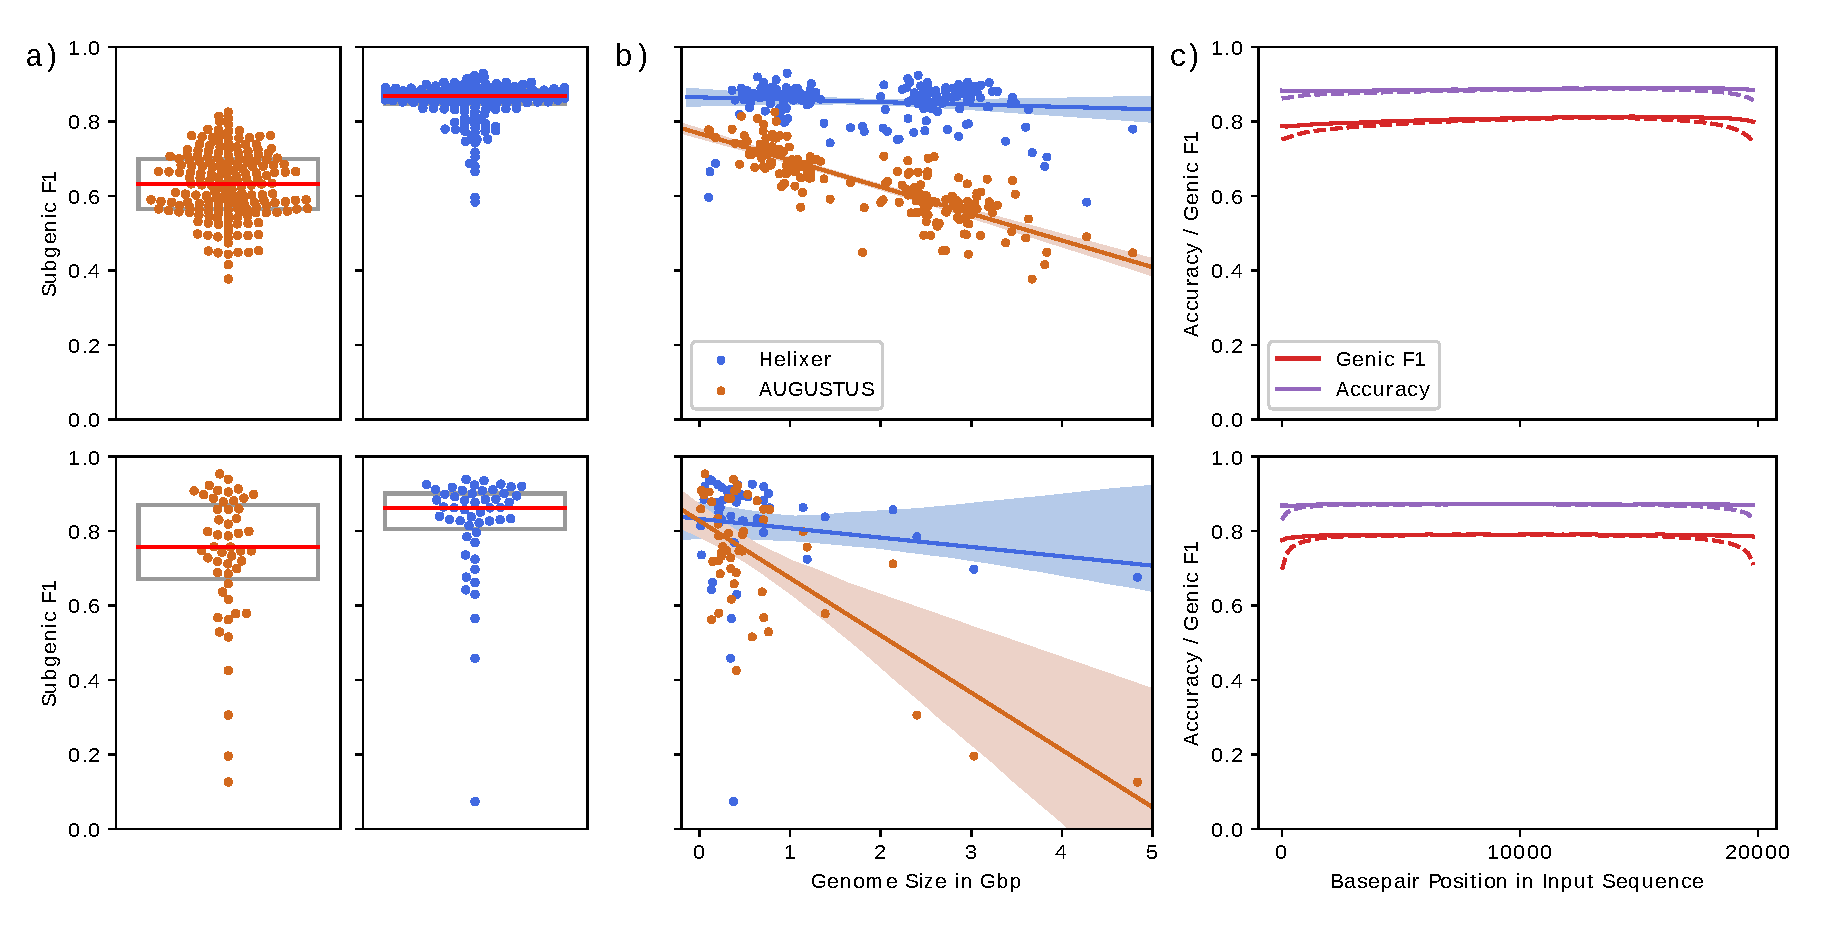
\includegraphics[width=\textwidth]{main_results}}
\caption{Main overall results and other investigations. The top and bottom rows
show the animal and plant data, respectively. Orange dots are for AUGUSTUS and 
the blue ones are for Helixer. {\bf a)} Swarm - and boxplots showing the Subgenic F1 
scores for all validation and test genomes. Each dot represents the prediction 
performace for one genome. The median prediction scores are shown by the red line. 
Details of how AUGUSTUS was used are given in Section \ref{sec:augustus}. {\bf b)} 
Scatterplots showing the prediction performances measured in Subgenic F1 by genome 
length. The regression line is shown with a 95\% confidence interval. {\bf c)} The 
average Genic F1 (in red) and basepair wise accuracy (in purple) with respect to 
the position in the 20,000 basepair long input sequences. The dashed line shows the 
same without overlapping. Each value is the average performance of a 200 basepair 
long subsection by one of the models of the final ensemble. 
See Section \ref{ssec:overlapping} of the 
Supplements for the effects of overlapping in individual species.}
\end{figure*}

\begin{table}[!t]
\processtable{Summary of Experimental Results\label{tab:results}} {
\begin{tabular}{@{}lll@{}}
\toprule & Animals & Plants\\
\midrule
AUGUSTUS & 0.632 & 0.757 \\
Dilated CNN Baseline & 0.666 &  0.802 \\
Best Helixer model & 0.77  & 0.833  \\
Best model + varied input length & 0.834  & - \\
Best model (+ varied input length) + overlapping &  0.844  & 0.843  \\
(Varied input length +) overlapping + ensembling & 0.868  & 0.863  \\
\botrule
\end{tabular}}{{\it Note:} Values are the median in Subgenic F1 across all 
validation and test genomes of the respective group. Varied input length was only 
used in the animal case. The best model was chosen out of the eight models of the 
ensemble for having the best performance on the validation set of the training genomes.}
\end{table}

\section{Results}
Figure \ref{fig:main_results}a shows the side-by-side comparison of the distribution 
of performances on all non-training genomes in the animal and plant case by Subgenic 
F1. In the case of Helixer, these scores represent cross-species predictions. We 
also compare the median performances of different configurations of Helixer with 
AUGUSTUS and a dilated CNN baseline in Table \ref{tab:results}. The results show a 
clear improvement over the AUGUSTUS both in higher median performance and reduced spread. We also 
significantly outperform a baseline constructed of a dilated CNN architecture.

Our models, however, tend to perform less well for the very smallest and largest 
genomes or species that are phylogenetically the furthest away from our training 
genomes. This is the case for both animals and plants and is visualized in
Figures S\ref{supfig:phylogeny_f1_animals} and S\ref{supfig:phylogeny_f1_plants}. 
We do not, for example, consistently predict very well on the 
algae nor on the non-avian reptiles. While one of the algae were included 
in our training genomes it accounted for a tiny proportion of the total training 
data and the non-avian reptiles were not included at all.
 
AUGUSTUS outperforms us on some of the smallest genomes, but falls off much more 
drastically as the genomes get larger. The difference in prediction quality is 
especially strong for mammals, which tend to have big genomes with very long genes 
as well as the largest plants. Figures S\ref{supfig:phylogeny_differences_animals} 
and S\ref{supfig:phylogeny_differences_plants} display the comparison to AUGUSTUS 
by phylogenetic position.

Two techniques were used during inference to improve performance and limit model 
bias. The usage of longer input lengths helped especially for genomes that tend to 
have longer genes and was enabled by our model architecture being a relatively 
simple BLSTM stack without any fully connected layers on top. We also constructed the 
final predictions out of a overlapping ones, which greatly helped to reduce 
prediction bias in most genomes. To our knowledge, neither technique has been used 
before in a model developed for gene annotation. 

\begin{figure*}[!h]
\label{fig:cov_example_main}
\centerline{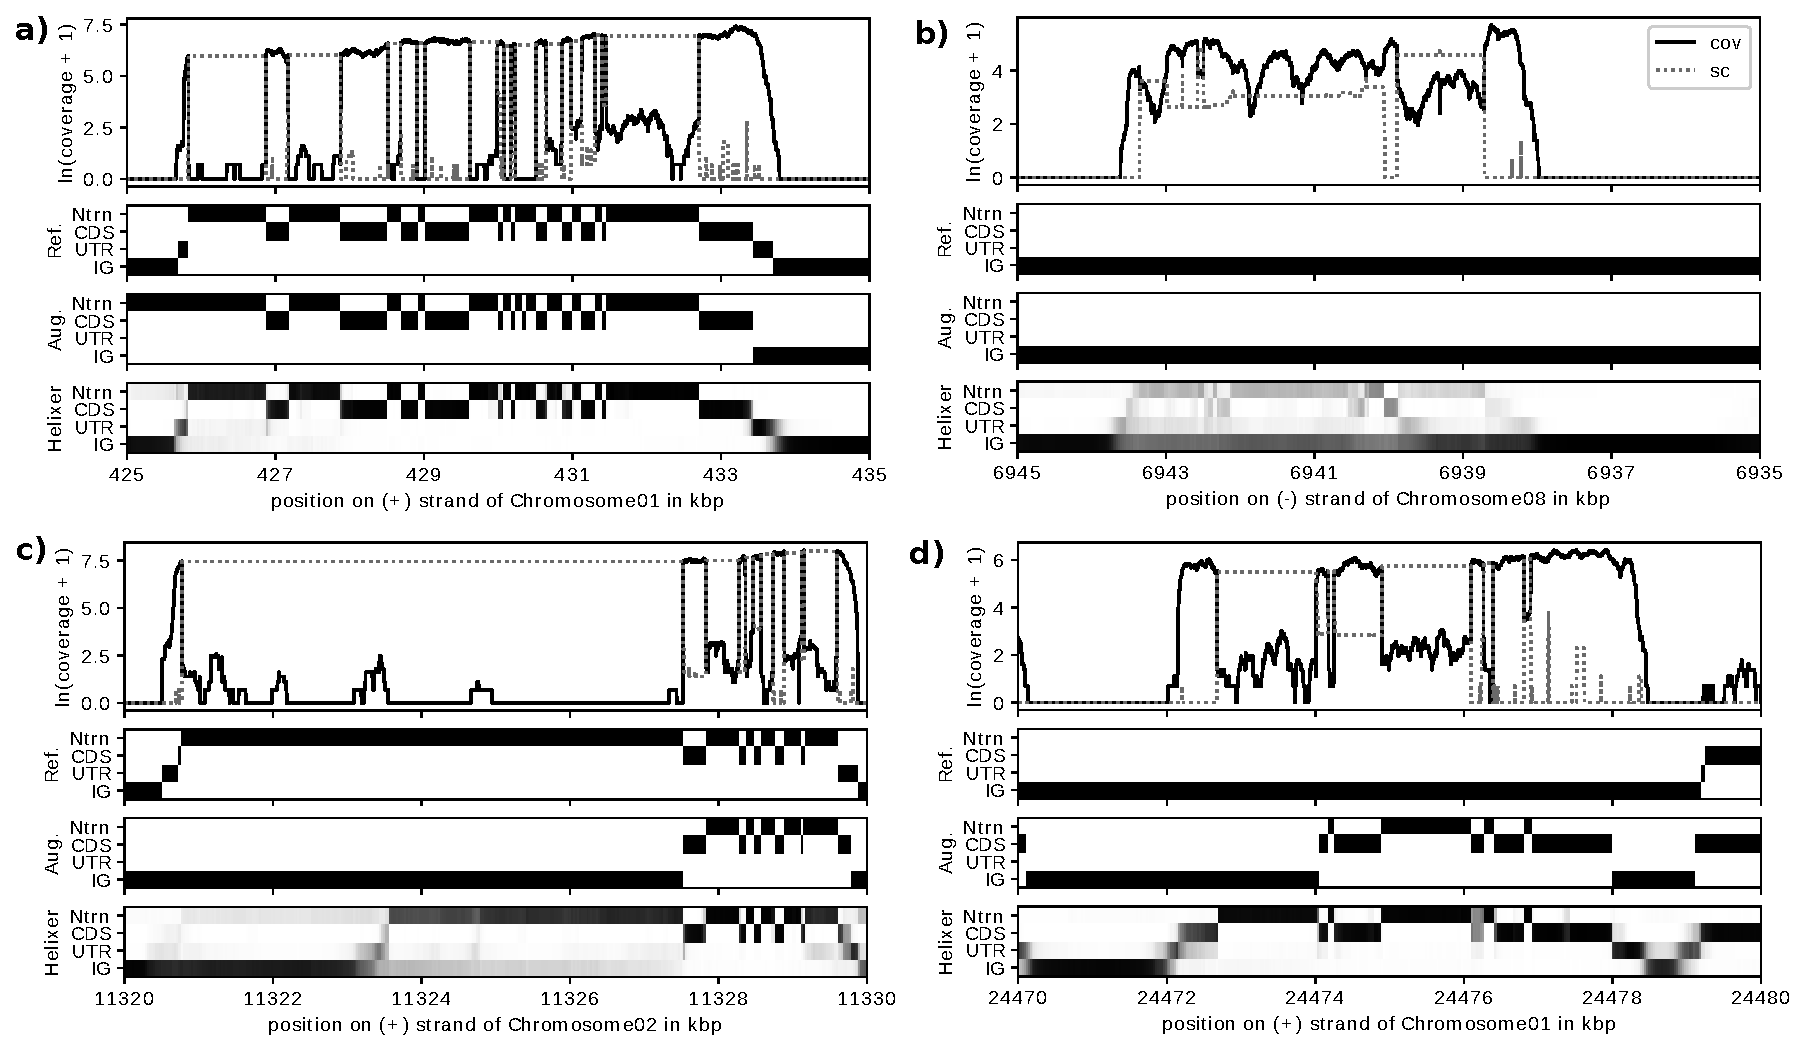
\includegraphics[width=\textwidth]{cov_example_main}}
\caption{Four example helixer predictions in the context of RNAseq data, the reference,
and AUGUSTUS' prediction for {\it M. esculenta}. The examples were chosen so
that {\bf a)} Helixer had high accuracy against the reference and the reference
was supported by the RNAseq data, {\bf b)} Helixer had high accuracy but the 
reference was not supported by the RNAseq data, {\bf c)} Helixer had low accuracy
and the reference was supported by the RNAseq data, and {\bf d)} helixer had low
accuracy but the reference was not supported by RNAseq data. Feasibility for visualization was
a major secondary consideration. Each subplot shows from top to
bottom i) the natural log of the coverage (``cov", solid) and spliced coverage 
(``sc", dotted) + 1, ii) the reference annotation in matrix form, iii) 
AUGUSTUS' predictions in matrix form, and iv) Helixer's predictions. The reference
and AUGUSTUS have either 0 (white) or 1 (black) for each base pair and category, while
Helixer emits a probability from 0-1 represented via gray-scale. ``Ntrn" stand
for intron, and ``IG" stands for intergenic.
}
\end{figure*}

To make an independent qualitative and quantitative evaluation of
performance we compared Helixer predictions, AUGUSTUS predictions and the
reference to RNAseq coverage data. Evaluation with RNAseq data was performed for
three each of animal and plant species. RNAseq coverage provides support for an 
exonic annotation (UTR or CDS), spliced coverage provides support for an 
annotation of intron, and neither coverage nor spliced coverage is expected 
for intergenic annotations. Looking at selected subsequences (Figure \ref{fig:cov_example_main}) % and supplemental figures.
we identified cases where RNAseq supported a) both the annotations of the reference 
and Helixer, b) neither, c) the reference, but not Helixer,
and d) Helixer, but not the reference. 

Helixer models do not yet have postprocessing
to make finalized single predictions, but instead output base-wise probabilities.
We see that the model exhibits higher uncertainty around transitions between annotation 
classes, for instance between UTR and CDS, or more dramatically between UTR and 
intergenic even where Helixer predictions closely match the reference and RNAseq data (a). 
Helixer's uncertainty around transitions from UTR to intergenic regions may relate to a
fundamentally harder problem (there is no conserved motif at the site as is observed
for splice sites and start/stop codons), lack of a precise one 
base pair biological site \citep{carninci2006genome,hon2013quantification}
or noise in the reference, which we observed relative to the RNAseq data 
(Figures S\ref{supfig:UTRs_animals}-\ref{supfig:UTRs_plants}). % supplemental UTR figures, 1/species

Helixer models also sometimes showed uncertainty for larger regions.
In some cases where Helixer did not receive RNAseq support for its highest probability
annotation, it assigned a low but non-trivial probability to the RNAseq-supported 
exon/intron pattern (Figures \ref{fig:cov_example_main}b-c, S\ref{supfig:cov_example_02}c). However, in the extreme,
there are cases where the Helixer model exhibits substantial indecision or confusion 
and shifts gradually between classes with no single class receiving a high probability 
for extended stretches (Figures S\ref{supfig:cov_example_02}c-d). 
Notably, in one of the examples (Figure S\ref{supfig:cov_example_02}d)
the RNAseq shows evidence of alternative splicing; 
and in another (Figure S\ref{supfig:cov_example_02}c) Helixer's
prediction falls between that of the reference and of AUGUSTUS.

\begin{figure}[hbt]
\label{fig:average_vs_augustus}
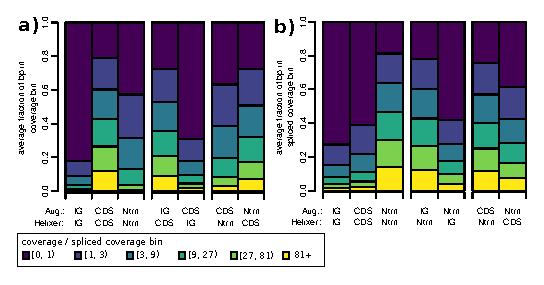
\includegraphics[width=8.6cm]{average_vs_augustus} 
\caption{Fraction of bp with color-indicated {\bf a)} coverage and {\bf b)} spliced coverage of genomic positions 
broken down by the confusion matrix of AUGUSTUS' and Helixer's predictions. Categories 
are only displayed if they can be meaningfully compared by examining a) coverage or b) spliced
coverage. The displayed fractions are the averages of the individual fractions for the 
six RNAseq-evaluation species. The left-most bars show cases where the two tools agree, 
while the remaining bars show paired conflicts. ``Ntrn" stand
for intron, and ``IG" stands for intergenic.}
\end{figure}

Coverage and Spliced coverage were broken down by the confusion matrix of both
Helixer vs AUGUSTUS as well as Helixer vs the reference for all genomes (Figure \ref{fig:average_vs_augustus}). 
Where both tools agree on far left in the figure, coverage and spliced coverage closely matched expectations. 
Specifically for CDS:CDS and UTR:UTR most base pairs had some, and many
had moderate or high coverage. The same pattern was seen for intron:intron and spliced
coverage. Finally, intergenic:intergenic showed only a small fraction of base pairs with 
any of either coverage or spliced coverage. In all conflicts the amount of RNAseq support
fell between the cases where tools agreed, indicating that all options were at least
capable of finding weak-spots in the other annotations.

In cases of conflict, Helixer's predictions were substantially more consistent with
the RNAseq data than those of AUGUSTUS. Specifically, for base pairs where one tool predicted CDS and
the other intergenic or intron, there was more coverage when 
Helixer predicted CDS (Figure \ref{fig:average_vs_augustus}a). 
Similarly, for base pairs where one tool predicted intron and the other 
CDS or intergenic, there was more spliced coverage when Helixer predicted intron (Figure \ref{fig:average_vs_augustus}b). 
These patterns were consistent in direction but varied in magnitude in the individual species,
with the exception of {\it P. marinus} where Helixer and AUGUSTUS performed comparably
at differentiating between CDS and intron regions (Figure S\ref{supfig:each_sp_vs_augustus}).

RNAseq based comparison of Helixer and the reference was less clear cut.
Averaged across species, Helixer's predictions received slightly more support
than the reference when differentiating CDS, UTR and introns from intergenic;
however Helixer's predictions received slightly less support than the reference 
when differentiating CDS and UTR from introns (Figure S\ref{supfig:average_vs_ref}). 
Performance varies between individual
species, from {\it P. marinus}, where the reference receives more support
in every conflict, to {\it T. cacao}, where Helixer models receive equivalent
or more support in every conflict (Figure S\ref{supfig:each_sp_vs_ref}). Interestingly, these two
species were selected as examples where Helixer had poor Subgenic F1; 
for the former the RNAseq confirms relatively weak performance for Helixer, while the 
for the latter RNAseq rather indicates a sub-par reference. 

\section{Discussion}
With Helixer, we introduce a novel, deep-learning based framework for the development 
of more effective tools for gene annotation prediction. 
Helixer outperforms AUGUSTUS on base pair wise metrics and on 
consistency with independent RNASeq data while also predicting cross-species for a wide range of  
genomes with one model. 

We include trained models for plants and animals which achieve 
high prediction accuracy on gene annotation for broad 
phylogenetic groups (land plants and vertebrates, respectively).
Within these groups, this eliminates the dependency on retraining and the
expertise and data required therefore. Production of comparable, single-method
annotations for broad groups has the potential to greatly facilitate downstream
analyses; for instance it could avoid some of the inconsistency and errors that
are otherwise seen in RNAseq analyses when different annotations are used 
\citep{zhao2015comprehensive,torres2016robust}.

We found our models to be highly sensitive to the training genomes we chose. A 
different set could lead to a significant shift in strengths and weaknesses of the 
model and a larger and more spread out set of high quality genomes could also result 
in a wider range of genomes with decent predictions. For this, more computational 
resources would be required. Simply training with a similar amount of data, 
but for a different group (e.g. invertebrates of fungi) could also be used to 
increase the functional predictive range. 

An avenue for future research could be the addition of RNASeq data as additional 
input. This would bring Helixer on even footing with current tools and could lead 
to real world applicable performance improvements if the results of this work are 
any indication, as deep learning has been shown to excel in a multimodal settings 
\citep{ching2018opportunities}.

Finally, development of a post-processing method
to go from base pair wise predictions to integrated predictions for whole 
transcripts at each loci could both further improve performance and would
greatly increase real world applications.
\section*{Funding}
This work has been supported by the Deutsche Forschungsgemeinschaft (DFG, German Research Foundation) 
under Germany's Excellence Strategy--EXC-2048/1--Project ID: 390686111.\vspace*{-12pt}
\section*{Acknowledgements}
We are grateful for the computational support and GPU access provided by
the de.NBI cloud, and by both the Centre for Information and Media Technology (ZIM)
and the Institute of Quantitative and Theoretical Biology at Heinrich Heine University.

\bibliographystyle{natbib}
\bibliography{literature}
% place holders for supplemental things
% ori version was grepped out of supplements, then
% :'<,'>s/^/\\begin{supfig}/g
% :'<,'>s/$/\\end{supfig}/g
% and similar for tables/sections
% tables

\begin{suptab}\label{suptab:downloads_animals}\end{suptab}
\begin{suptab}\label{suptab:downloads_plants}\end{suptab}
\begin{suptab}\label{suptab:generalization_animals}\end{suptab}
\begin{suptab}\label{suptab:generalization_plants}\end{suptab}
\begin{suptab}\label{suptab:params}\end{suptab}
\begin{suptab}\label{suptab:classweights}\end{suptab}
\begin{suptab}\label{suptab:rnaseq_samples}\end{suptab}
\begin{suptab}\label{suptab:bioinfo_params}\end{suptab}
\begin{suptab}\label{suptab:prediction_lengths}\end{suptab}
\begin{suptab}\label{suptab:genome_stats}\end{suptab}
\begin{suptab}\label{suptab:dcnn_xval}\end{suptab}
\begin{suptab}\label{suptab:dcnn_params}\end{suptab}
% figures
\begin{supfig}\label{supfig:phylogeny_f1_animals}\end{supfig}
\begin{supfig}\label{supfig:phylogeny_differences_animals}\end{supfig}
\begin{supfig}\label{supfig:phylogeny_f1_plants}\end{supfig}
\begin{supfig}\label{supfig:phylogeny_differences_plants}\end{supfig}
\begin{supfig}\label{supfig:rna_select_animals}\end{supfig}
\begin{supfig}\label{supfig:rna_select_plants}\end{supfig}
\begin{supfig}\label{supfig:overlapping_animals}\end{supfig}
\begin{supfig}\label{supfig:overlapping_plants}\end{supfig}
\begin{supfig}\label{supfig:cov_example_02}\end{supfig}
\begin{supfig}\label{supfig:cov_example_03}\end{supfig}
\begin{supfig}\label{supfig:UTRs_animals}\end{supfig}
\begin{supfig}\label{supfig:UTRs_plants}\end{supfig}
\begin{supfig}\label{supfig:average_vs_ref}\end{supfig}
\begin{supfig}\label{supfig:each_sp_vs_augustus}\end{supfig}
\begin{supfig}\label{supfig:each_sp_vs_ref}\end{supfig}
% sections
\begin{supsec}\label{ssec:data_prep}\end{supsec}
\begin{supsec}\label{ssec:generalization}\end{supsec}
\begin{supsec}\label{ssec:hyperparameters}\end{supsec}
\begin{supsec}\label{ssec:rnaseq_setup}\end{supsec}
\begin{supsec}\label{ssec:longer}\end{supsec}
\begin{supsec}\label{ssec:overlapping}\end{supsec}
\begin{supsec}\label{ssec:training_data}\end{supsec}
\begin{supsec}\label{ssec:dcnn}\end{supsec}
\begin{supsec}\label{ssec:rnaseq_eval}\end{supsec}
% datasets
\begin{supdata}\label{supdata:metadata}\end{supdata}  % just a placeholder for the CSV and where it's referenced


\end{document}
